\section{Durchführung}
\label{sec:Durchfuehrung}
\begin{figure}
    \centering
    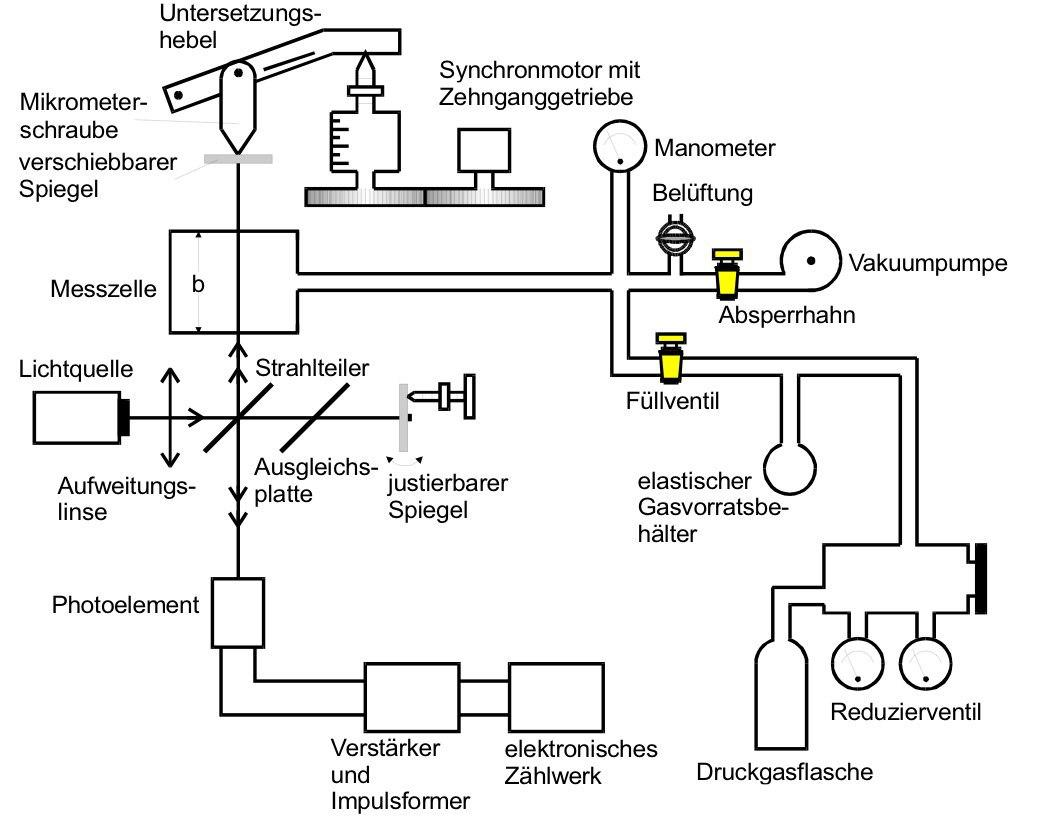
\includegraphics[width=0.6\textwidth]{bilder/aufbau.jpg}
    \caption{Messapperatur \cite[9]{anleitung}}
\end{figure}
\subsection{Justierung}
Zunächst muss die Apperatur justiert werden. Dafür werden die beiden hellsten Strahlen die aus dem
Interometer austreffen zur Deckung gebracht. Ein Justierspiegel wird dazu verwendet, um die Deckung auf deiner Jilfsmattscheibe zu erziehlen.
Danach muss das Photoelement, was zur Zählung der Maximas verwendet wird, auf die richtige Höhe 
eingestellt werden, sodass das Interferenzbild genau auf dem Eintrittspalt entsteht.\\
\subsection{Messung aufnehmen}
Um nun die Messung zu starten kann einer der beiden Spiegel mithilfe ines Motors über eine
Mikrometerschraube bewegt werden. Die Geschwindigkeit muss auf das Photoelement angepasst sein, um alle Impuls aufnehmen zu können.
Die Spiegelverschiebung $\Delta d$, sowie die Anzah der Interferenzmaxima $z$ wird notiert.
Die Messung wird 10mal durchgeführt.
\subsection{Brechnungsindex}
Ziel ist es den Brechnungsindex von Luft zu messen. Nun werden keine Spiegel mehr bewegt und der
Motor kann ausgeschaltet werden. Eine Messzelle wird nun auf einen Druck $p$ evakuiert.
Beim langsamen wiedereinlassen der Luft, zählt man nun erneut die Anzahl $z$ der Interferenzen.
Der sich einstellende Druck $p_0$ wird nun als Normaldruck angenommen.
